\documentclass[a4paper,twoside]{article}
\usepackage{blindtext}  
\usepackage{geometry}

% Chinese support
\usepackage[UTF8, scheme = plain]{ctex}

% Page margin layout
\geometry{left=2.3cm,right=2cm,top=2.5cm,bottom=2.0cm}


\usepackage{listings}
\usepackage{xcolor}
\usepackage{geometry}
\usepackage{amsmath}
\usepackage{float}
\usepackage{hyperref}

\usepackage{graphics}
\usepackage{graphicx}
\usepackage{epsfig}
\usepackage{float}
\usepackage{wrapfig}

\usepackage{algorithm}
\usepackage[noend]{algpseudocode}

\usepackage{booktabs}
\usepackage{threeparttable}
\usepackage{longtable}
\usepackage{listings}
\usepackage{tikz}
\usepackage{multicol}

\usepackage{caption}
\usepackage{subcaption}

% cite package, to clean up citations in the main text. Do not remove.
\usepackage{cite}

\usepackage{color,xcolor}

%% The amssymb package provides various useful mathematical symbols
\usepackage{amssymb}
%% The amsthm package provides extended theorem environments
\usepackage{amsthm}
\usepackage{amsfonts}
\usepackage{enumerate}
\usepackage{enumitem}
\usepackage{listings}

\usepackage{textcomp}

\usepackage{indentfirst}
\setlength{\parindent}{2em} % Make two letter space in the first paragraph
\usepackage{setspace}
\linespread{1.5} % Line spacing setting
\usepackage{siunitx}
\setlength{\parskip}{0.5em} % Paragraph spacing setting

% \usepackage[contents =22920202204622, scale = 10, color = black, angle = 50, opacity = .10]{background}

\renewcommand{\figurename}{图}
\renewcommand{\lstlistingname}{代码} 
\renewcommand{\tablename}{表格}
\renewcommand{\contentsname}{目录}
\floatname{algorithm}{算法}

\graphicspath{ {images/} }

%%%%%%%%%%%%%
\newcommand{\StudentNumber}{22920202204622}  % Fill your student number here
\newcommand{\StudentName}{熊恪峥}  % Replace your name here
\newcommand{\PaperTitle}{实验(五)}  % Change your paper title here
\newcommand{\PaperType}{计算机网络} % Replace the type of your report here
\newcommand{\Date}{2022年12月1日}
\newcommand{\College}{信息学院}
\newcommand{\CourseName}{计算机网络}
%%%%%%%%%%%%%

%% Page header and footer setting
\usepackage{fancyhdr}
\usepackage{lastpage}
\pagestyle{fancy}
\fancyhf{}
% This requires the document to be twoside
\fancyhead[LO]{\texttt{\StudentName }}
\fancyhead[LE]{\texttt{\StudentNumber}}
\fancyhead[C]{\texttt{\PaperTitle }}
\fancyhead[R]{\texttt{第{\thepage}页,共\pageref*{LastPage}页}}


\title{\PaperTitle}
\author{\StudentName}
\date{\Date}

\lstset{
	basicstyle          =   \sffamily,          % 基本代码风格
	keywordstyle        =   \bfseries,          % 关键字风格
	commentstyle        =   \rmfamily\itshape,  % 注释的风格,斜体
	stringstyle         =   \ttfamily,  % 字符串风格
	flexiblecolumns,                % 别问为什么,加上这个
	numbers             =   left,   % 行号的位置在左边
	showspaces          =   false,  % 是否显示空格,显示了有点乱,所以不现实了
	numberstyle         =   \zihao{-5}\ttfamily,    % 行号的样式,小五号,tt等宽字体
	showstringspaces    =   false,
	captionpos          =   t,      % 这段代码的名字所呈现的位置,t指的是top上面
	frame               =   lrtb,   % 显示边框
}

\lstdefinestyle{PythonStyle}{
	language        =   Python, % 语言选Python
	basicstyle      =   \zihao{-5}\ttfamily,
	numberstyle     =   \zihao{-5}\ttfamily,
	keywordstyle    =   \color{blue},
	keywordstyle    =   [2] \color{teal},
	stringstyle     =   \color{magenta},
	commentstyle    =   \color{red}\ttfamily,
	breaklines      =   true,   % 自动换行,建议不要写太长的行
	columns         =   fixed,  % 如果不加这一句,字间距就不固定,很丑,必须加
	basewidth       =   0.5em,
}

\definecolor{keycolor}{RGB}{172, 42, 42}
\definecolor{mbleu}{RGB}{64,96,127}
\definecolor{vimvert}{RGB}{46, 139, 87}

\lstdefinestyle{MakefileBaseStyle}{
basicstyle=\ttfamily\scriptsize\color{black!90},%
stringstyle=\itshape\color{magenta},%
showstringspaces=false,%
keywordstyle=\bfseries\color{keycolor},%
commentstyle=\color{blue}\slshape,%
framexleftmargin=1mm,%
backgroundcolor=\color{black!2},%
}

\lstdefinestyle{MakefileStyle}{
	otherkeywords={.SUFFIXES},
	morekeywords={SUFFIX, CPP_,},
	moredelim=[is][\color{mbleu}]{/*}{*/},
	style=MakefileBaseStyle,%
	morecomment=[l][commentstyle]{\#},%
	emphstyle={\color{vimvert}},%
	moredelim=[s][\color{vimvert}]{\$(}{)}%
}

\lstdefinestyle{CppStyle}{
	language        =   c++,
	basicstyle      =   \zihao{-5}\ttfamily,
	numberstyle     =   \zihao{-5}\ttfamily,
	keywordstyle    =   \color{blue},
	keywordstyle    =   [2] \color{teal},
	stringstyle     =   \color{magenta},
	commentstyle    =   \color{red}\ttfamily,
	breaklines      =   true,   % 自动换行,建议不要写太长的行
	columns         =   fixed,  % 如果不加这一句,字间距就不固定,很丑,必须加
	basewidth       =   0.5em,
}

\algnewcommand\algorithmicinput{\textbf{Input:}}
\algnewcommand\algorithmicoutput{\textbf{Output:}}
\algnewcommand\Input{\item[\algorithmicinput]}%
\algnewcommand\Output{\item[\algorithmicoutput]}%

\usetikzlibrary{positioning, shapes.geometric}

% 流程图定义基本形状
\tikzstyle{startstop} = [rectangle, rounded corners, minimum width = 2cm, minimum height=1cm,text centered, draw = black]
\tikzstyle{io} = [trapezium, trapezium left angle=70, trapezium right angle=110, minimum width=2cm, minimum height=1cm, text centered, draw=black]
\tikzstyle{process} = [rectangle, minimum width=3cm, minimum height=1cm, text centered, draw=black]
\tikzstyle{decision} = [diamond, aspect = 3, text centered, draw=black]
% 箭头形式
\tikzstyle{arrow} = [->,>=stealth]

\newtheorem{assumption}{Assumption}[section]

\begin{document}
	
%%%%%%%%%%%%%%%%%%%%%%%%%%%%%%%%%%%%%%%%%%%%
\makeatletter % change default title style
\renewcommand*\maketitle{%
	\begin{center} 
		\bfseries  % title 
		{\LARGE \@title \par}  % LARGE typesetting
		\vskip 1em  %  margin 1em
		{\global\let\author\@empty}  % no author information
		{\global\let\date\@empty}  % no date
		\thispagestyle{empty}   %  empty page style
	\end{center}%
	\setcounter{footnote}{0}%
}
\makeatother
%%%%%%%%%%%%%%%%%%%%%%%%%%%%%%%%%%%%%%%%%%%%
	
	
\thispagestyle{empty}

\vspace*{1cm}

\begin{figure}[h]
	\centering
	
\includegraphics[width=4.0cm]{logo.png}
\end{figure}

\vspace*{1cm}

\begin{center}
	\Huge{\textbf{\PaperType}}
	
	\Large{\PaperTitle}
\end{center}

\vspace*{1cm}

\begin{table}[h]
	\centering	
	\begin{Large}
		\renewcommand{\arraystretch}{1.5}
		\begin{tabular}{p{3cm} p{5cm}<{\centering}}
			姓\qquad 名 & \StudentName  \\
			\hline
			学\qquad号 & \StudentNumber \\
			\hline
			日\qquad期 & \Date  \\
			\hline
			学\qquad院 & \College  \\
			\hline
			课程名称 & \CourseName  \\
			\hline
		\end{tabular}
	\end{Large}
\end{table}

\newpage

\title{
	\Large{\textcolor{black}{\PaperTitle}}
}
	
	
\maketitle
	
\tableofcontents
 
\newpage
\setcounter{page}{1}

\begin{spacing}{1.2}

\section{任务1、TCP 正常连接观察}

在终端运行命令
\begin{center}
	\texttt{wget http://mba.xmu.edu.cn/favicon.ico --no-http-keep-alive}
\end{center}
传输上述URL中的文件,观察TCP连接的建立和关闭过程。抓取到的数据段如图~\ref{fig:tcpp}所示。
\begin{figure}[htb]
	\centering
	\caption{TCP数据段}
	\label{fig:tcpp}
	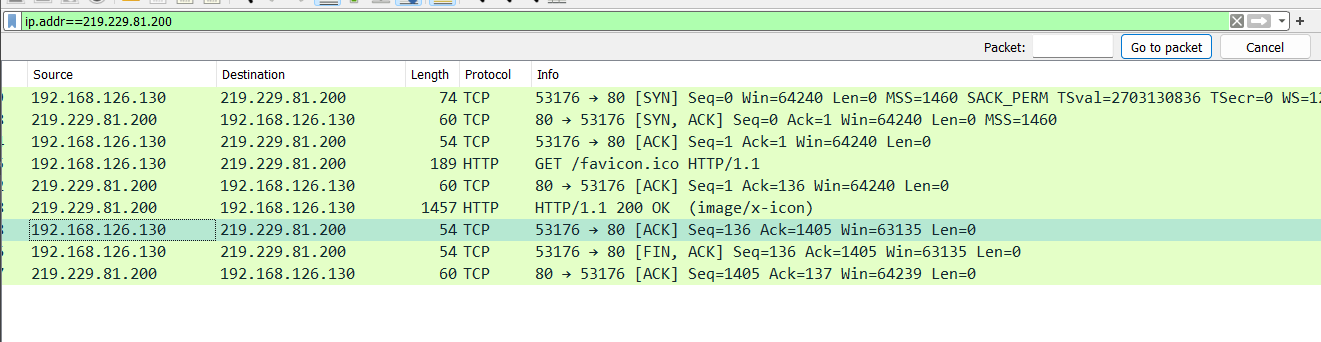
\includegraphics[width=0.8\textwidth]{tcp_packs.png}
\end{figure}
作出TCP流图,如图~\ref{fig:tcpflow}所示。
\begin{figure}[htb]
	\centering
	\caption{TCP流图}
	\label{fig:tcpflow}
	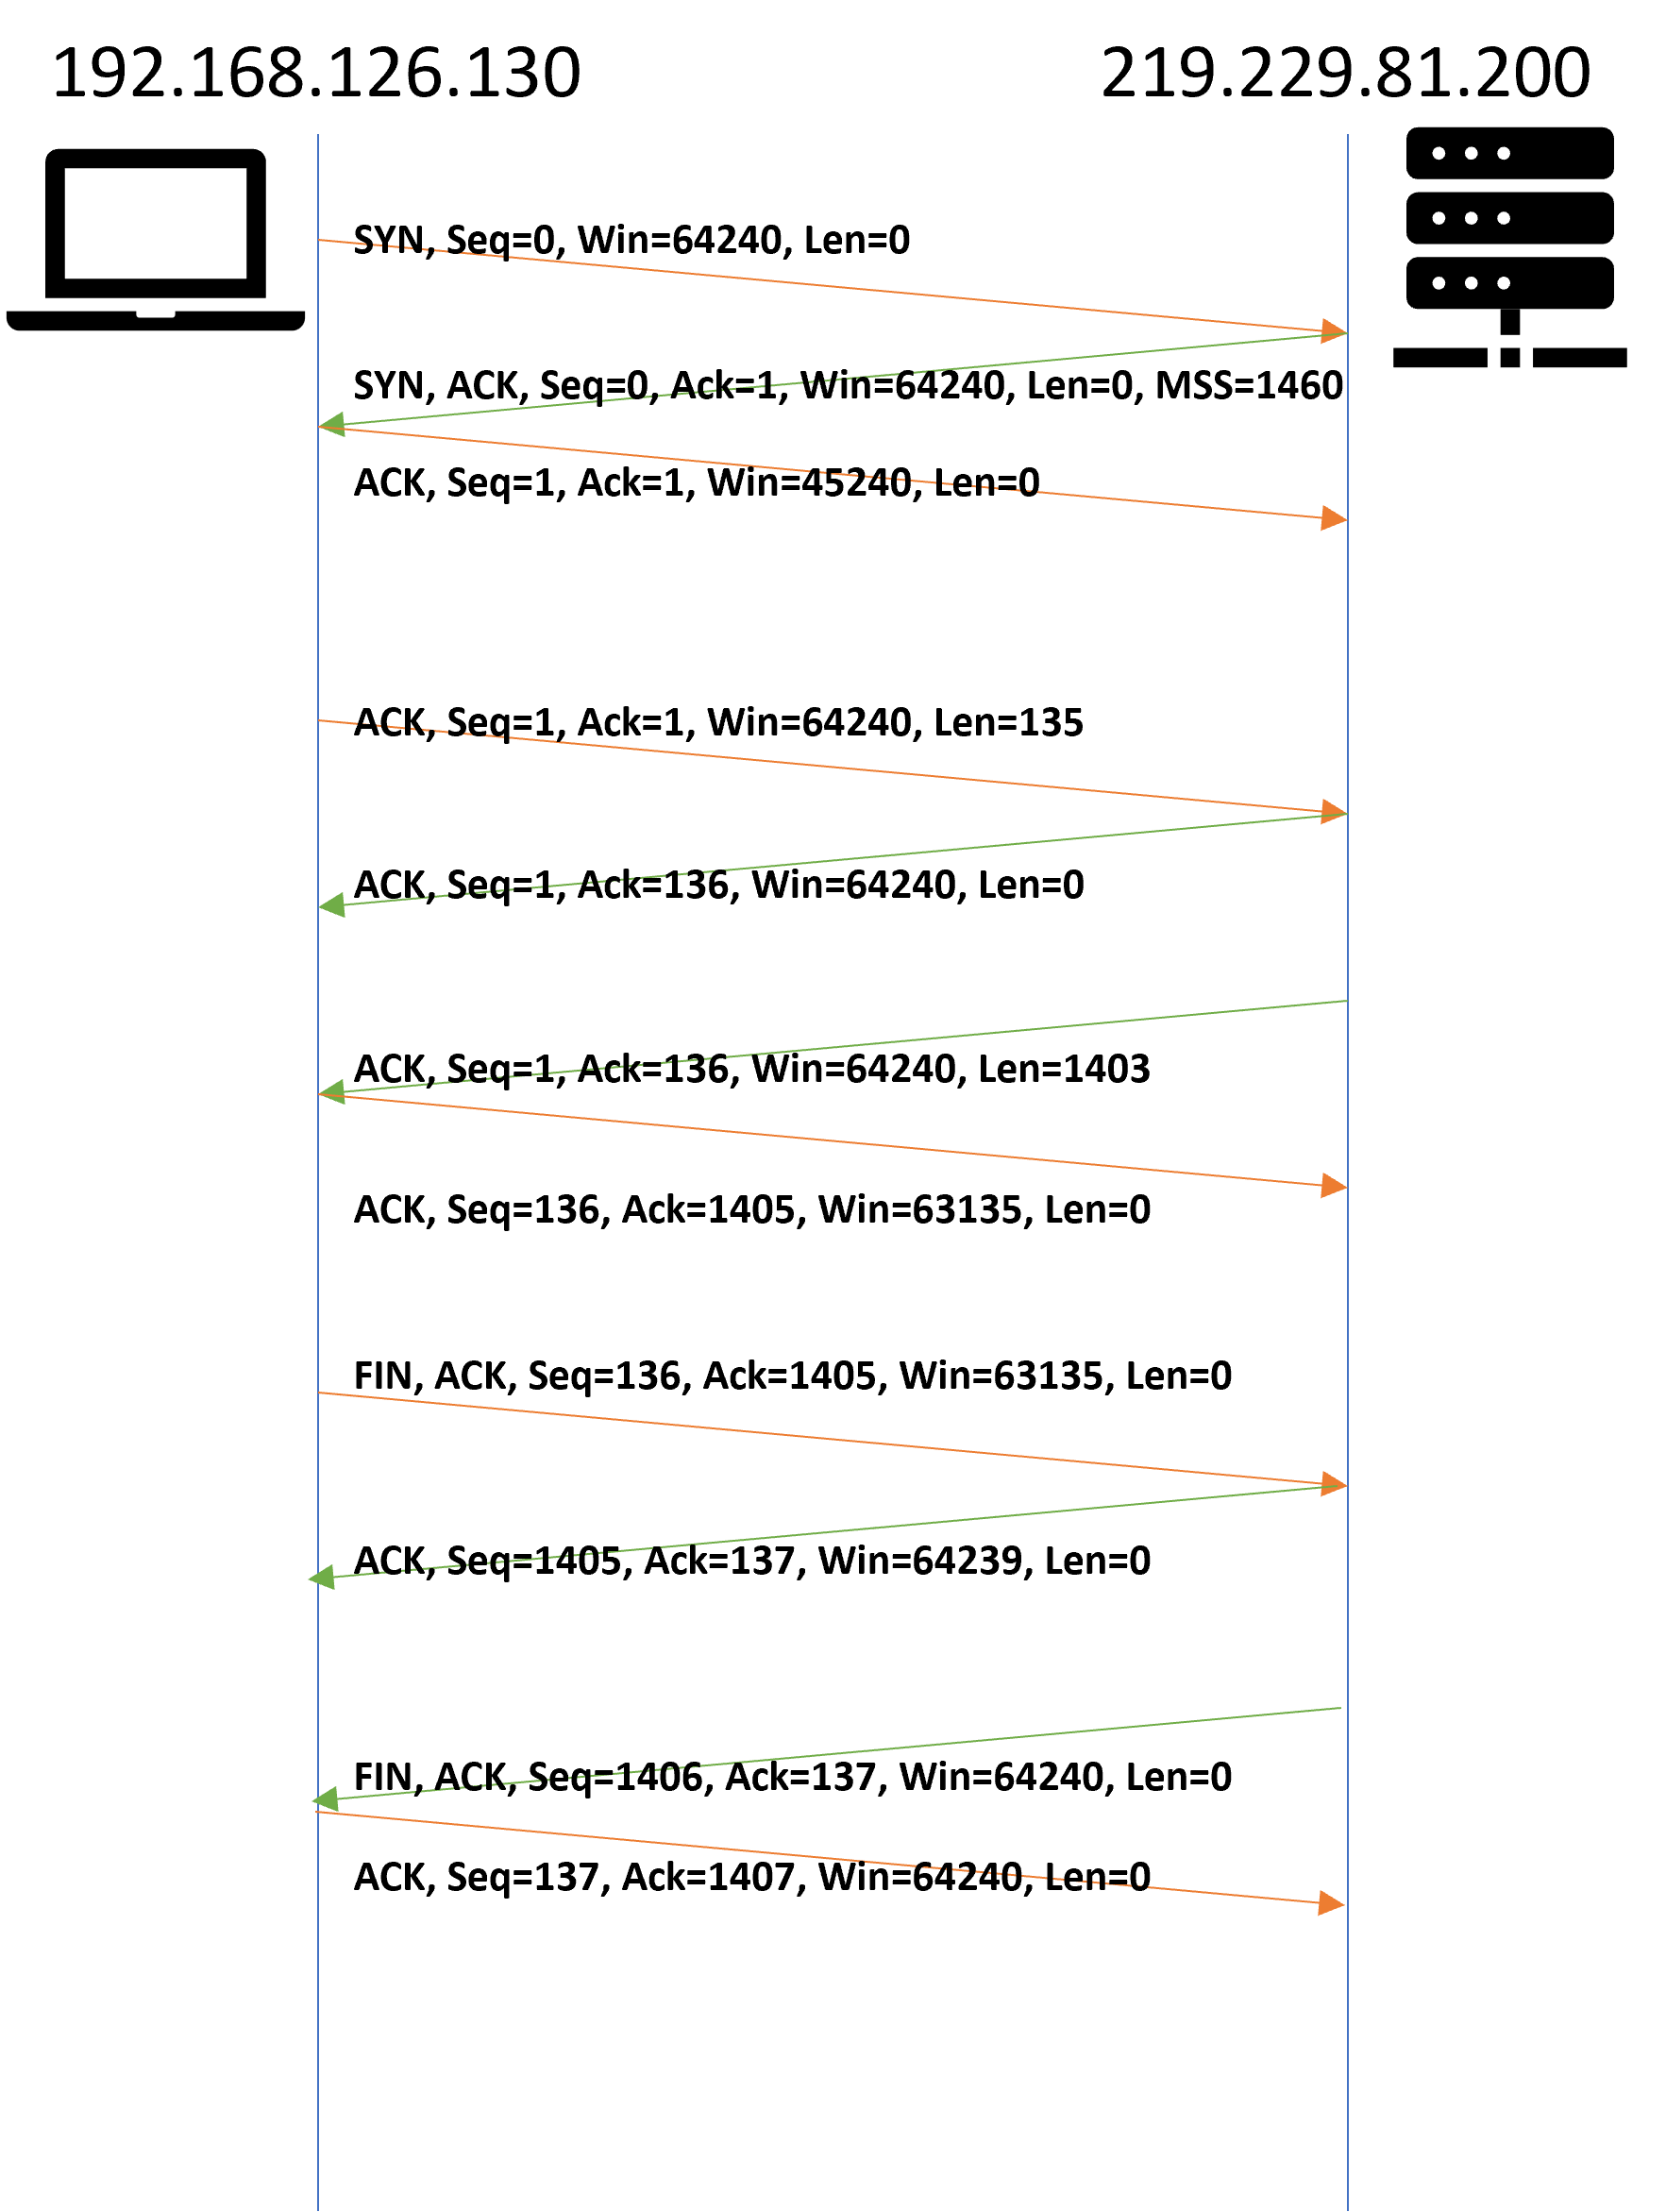
\includegraphics[width=0.5\textwidth]{tcp.png}
\end{figure}
由于Wireshark默认显示Sequence Number的相对值,因此这两个值都从0开始。实际上Sequence Number
由TCP连接的建立时随机生成,客户端从354954929开始,服务器端从794129432开始。如图~\ref{fig:tcpseq}所示。
\begin{figure}[htb]
	\centering
	\caption{TCP Sequence Number}
	\label{fig:tcpseq}
	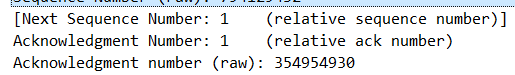
\includegraphics[width=0.5\textwidth]{realseq.png}
\end{figure}


\section{任务2、TCP异常传输观察分析}

\subsection{尝试连接未存活的主机或对未监听端口}

首先,随便指定一不存在的IP,使用wget访问该IP,例如\texttt{192.168.3.2}。如图~\ref{fig:badip}所示。
\begin{figure}[htb]
	\centering
	\caption{不存在的IP}
	\label{fig:badip}
	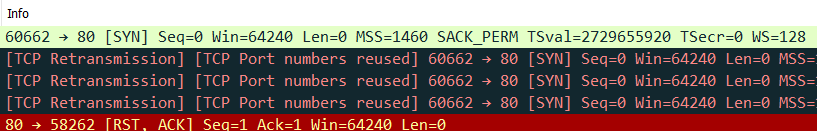
\includegraphics[width=0.8\textwidth]{badip.png}
\end{figure}
这样不存在的IP无法回应SYN请求,会引起不断地重传。Ubuntu中的重传次数默认为3。
以图中的重传为例,SYN发送后进行了三次重传,然后由于无响应发送了RST。可以计算时间间隔如
表~\ref{tbl:retrintv}和图~\ref{fig:retrintv}所示。
\begin{table}[htb]
	\centering
	\caption{时间间隔}
	\label{tbl:retrintv}
	\begin{tabular}{c|c|c|c}
		\toprule
		\hline
		$1\longrightarrow2$&$2\longrightarrow3$&$3\longrightarrow4$&$4\longrightarrow5$\\
		\hline
		1.013&2.015&4.095&6.400 \\
		\hline
		\bottomrule
	\end{tabular}
\end{table}
\begin{figure}[H]
	\centering
	\caption{时间间隔}
	\label{fig:retrintv}
	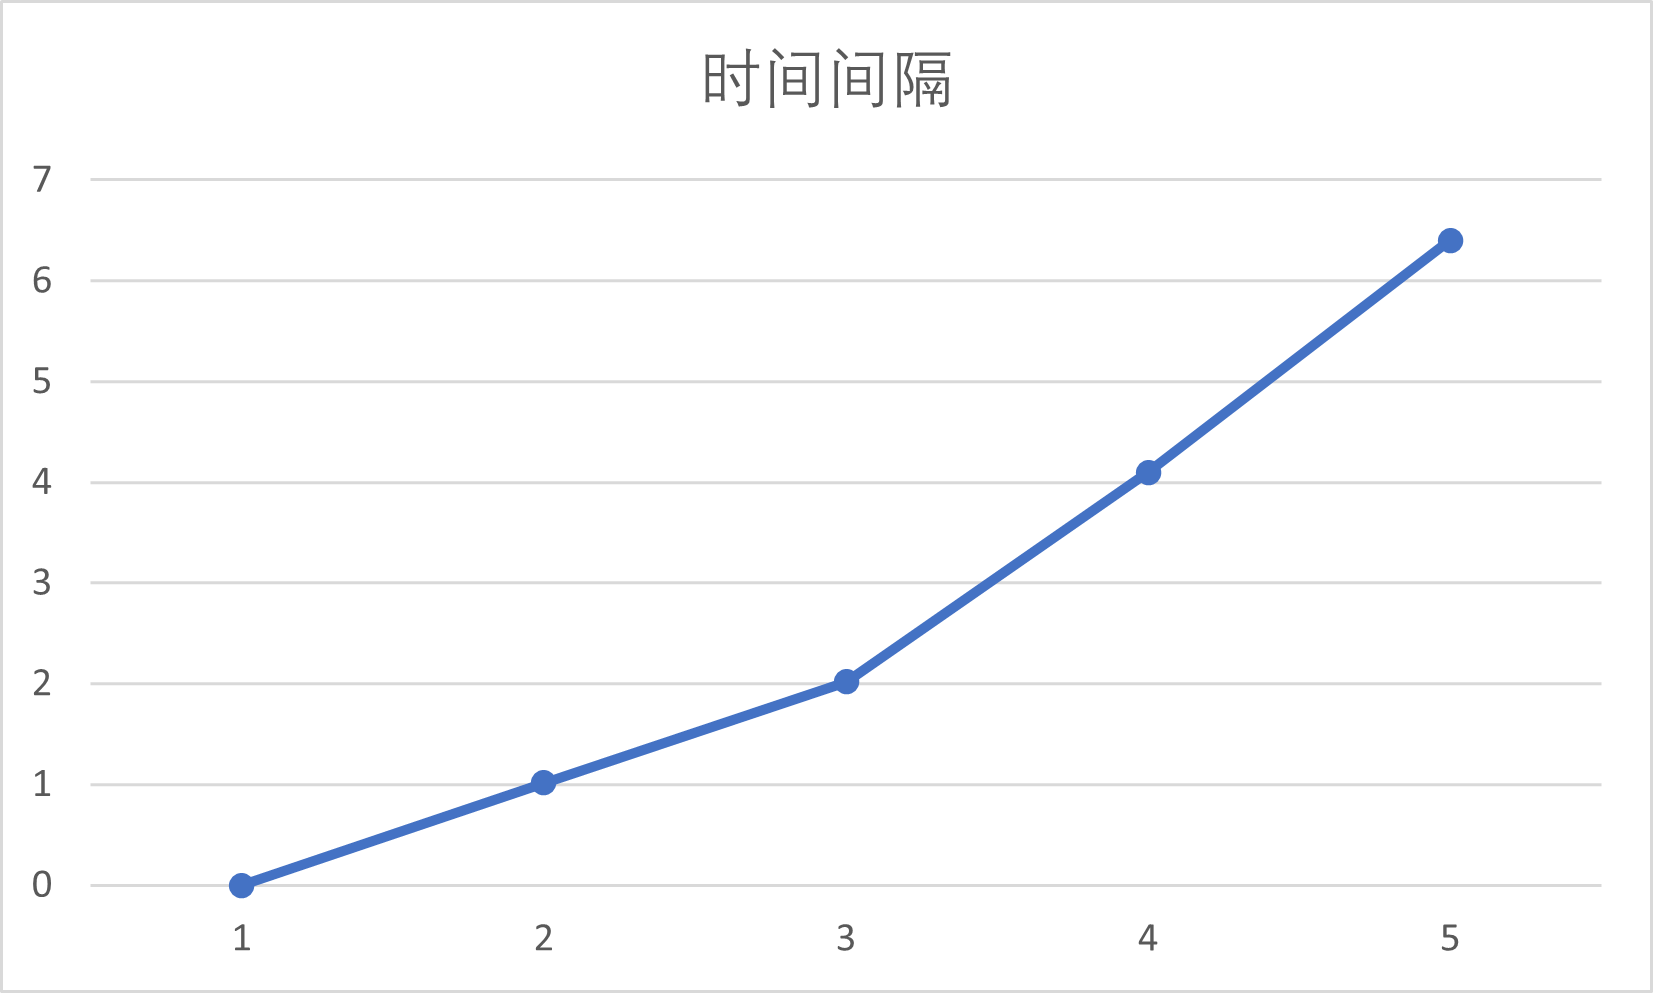
\includegraphics[width=0.5\textwidth]{interval.png}
\end{figure}
可以发现忽略测量误差,时间间隔是按$2^n$指数增长的。

借助RST,可以实现端口扫描。为针对TCP扫描,目前存在防御方式:
若发现网络中的某台设备进行了端口扫描,会将其加入黑名单。实现这种防御的原理是:每次TCP连接后会将信息记录到日志中,
当发现某IP多次连接设备的不同端口,就可以判断是TCP扫描,此时就可以将此IP加入黑名单。
为避免被TCP扫描抓到,可以采用SYN扫描,原理同样是利用了TCP三次握手,过程如下:
\begin{enumerate}
	\item 扫描端向目标端发送SYN请求建立连接
	\item 目标端收到请求后,回复ACK同意连接并同意发送SYN请求建立连接
	\item 扫描端收到后,发送RST拒绝建立连接。
\end{enumerate}

使用\texttt{nmap -sS localhost}命令扫描本机,如图~\ref{fig:nmap}所示。
\begin{figure}[htb]
	\centering
	\caption{nmap扫描}
	\label{fig:nmap}
	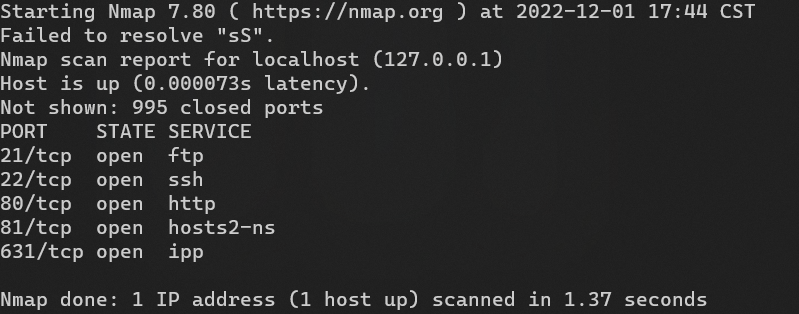
\includegraphics[width=0.6\textwidth]{nmap.png}
\end{figure}
它指出本机的SSH端口、FTP端口等是开放的。用Wireshark观察抓到的包,例如FTP端口21,如图~\ref{fig:ftp}所示。

可见,由于21端口是开放的,服务器得到SYN请求后会回复ACK准备建立连接。此时扫描程序得知了21端口是开放的,但
为了防止IP黑名单,就发送RST拒绝建立连接,此时服务器不能建立连接。因此无法记录客户IP进行屏蔽。这样就使得
扫描能够顺利完成。如图~\ref{fig:exist}所示。
\begin{figure}[htb]
	\centering
	\caption{21端口开放}
	\label{fig:exist}
	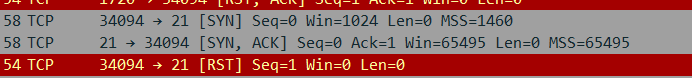
\includegraphics[width=0.6\textwidth]{exist.png}
\end{figure}
又例如端口587未开放。因此服务器就会发送RST,ACK表示收到请求但拒绝建立连接。扫描程序收到后,就会认为端口587
未开放。如图~\ref{fig:nexist}所示。
\begin{figure}[htb]
	\centering
	\caption{587端口未开放}
	\label{fig:nexist}
	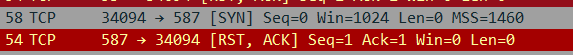
\includegraphics[width=0.6\textwidth]{nexist.png}
\end{figure}

\subsection{客户端发送了第一个 SYN 连接请求,服务器无响应}
\label{sec:client-syn}
为了简单地测试,可以通过下载远程的文件来测试。这里使用的文件如下:
\begin{center}
\texttt{https://mirrors.tuna.tsinghua.edu.cn/ubuntu-cdimage/releases/kinetic/\\ release/ubuntu-22.10-live-server-s390x.iso}
\end{center}
首先用\texttt{nslookup}命令获取下载该文件访问的IP地址,得知IP地址为\texttt{101.6.15.130}。
然后使用以下命令屏蔽IP地址发来的TCP SYN和ACK报文。
\begin{center}
\texttt{sudo iptables -I INPUT -s 101.6.15.130 -p tcp -m tcp --tcp-flags ALL SYN,ACK -j DROP}
\end{center}
这样其它的TCP内容可以正常通过,而建立连接的TCP SYN-ACK不能正常被收到。

然后使用\texttt{wget}命令下载文件,进行实验。首先,最初的SYN报文到达了服务器,然而服务器返回的
SYN-ACK无法被\texttt{wget}程序收到。因此导致了多次重传,如图~\ref{fig:syn}。
\begin{figure}[htb]
	\centering
	\caption{SYN-ACK重传}
	\label{fig:syn}
	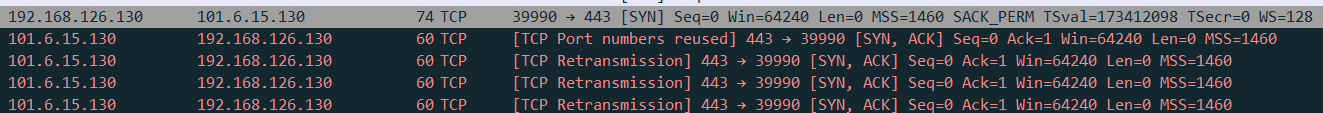
\includegraphics[width=0.6\textwidth]{syn.png}
\end{figure}
接下来,由于服务器相应被\texttt{iptables}丢弃,因此在指定时间之内收不到ACK报文的客户端认为
无从得知SYN是否被服务器收到,就会产生SYN请求的重传,如图~\ref{fig:synack}。
\begin{figure}[htb]
	\centering
	\caption{SYN重传}
	\label{fig:synack}
	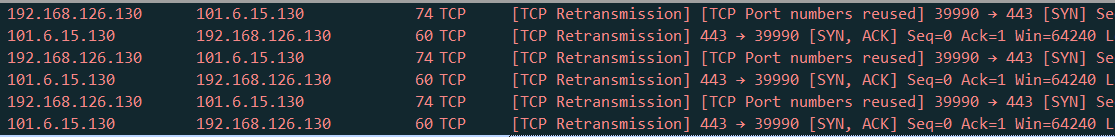
\includegraphics[width=0.6\textwidth]{synack.png}
\end{figure}

由于SYN-ACK无法到达,因此这个过程会反复持续多次。最终,\texttt{wget}程序无法建立连接
会发送RST,结束这一过程。如图~\ref{fig:rst}。
\begin{figure}[H]
	\centering
	\caption{RST}
	\label{fig:rst}
	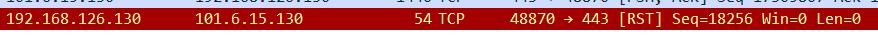
\includegraphics[width=0.6\textwidth]{rst.png}
\end{figure}


\section{任务3、拥塞控制}

\subsection{实验准备}

首先为了观察普通的拥塞控制算法,需要对使用的拥塞控制算法进行修改。所以
使用命令\texttt{sysctl -w net.ipv4.tcp\_congestion\_control=reno}修改拥塞控制算法为Reno。
然后在虚拟机设置中对带宽进行限制。如图~\ref{fig:bandwidth}所示。
\begin{figure}[H]
	\centering
	\caption{对带宽进行限制}
	\label{fig:bandwidth}
	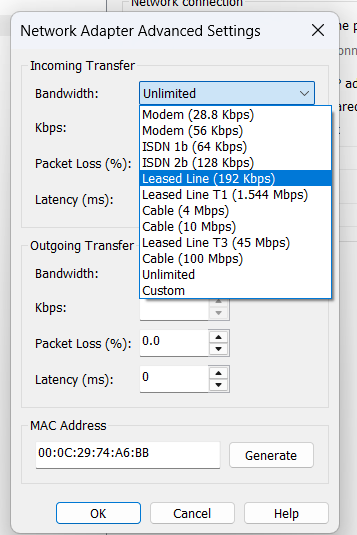
\includegraphics[width=0.3\textwidth]{bandwidth.png}
\end{figure}
这里为了使得效果明显,将带宽限制为192Kbps,然后下载第\ref{sec:client-syn}节中
提到的大文件。

\subsection{实验结果}

使用Wireshark中的IO Graph功能做出了如图~\ref{fig:io}所示的图表。
\begin{figure}[htb]
	\centering
	\caption{IO Graph}
	\label{fig:io}
	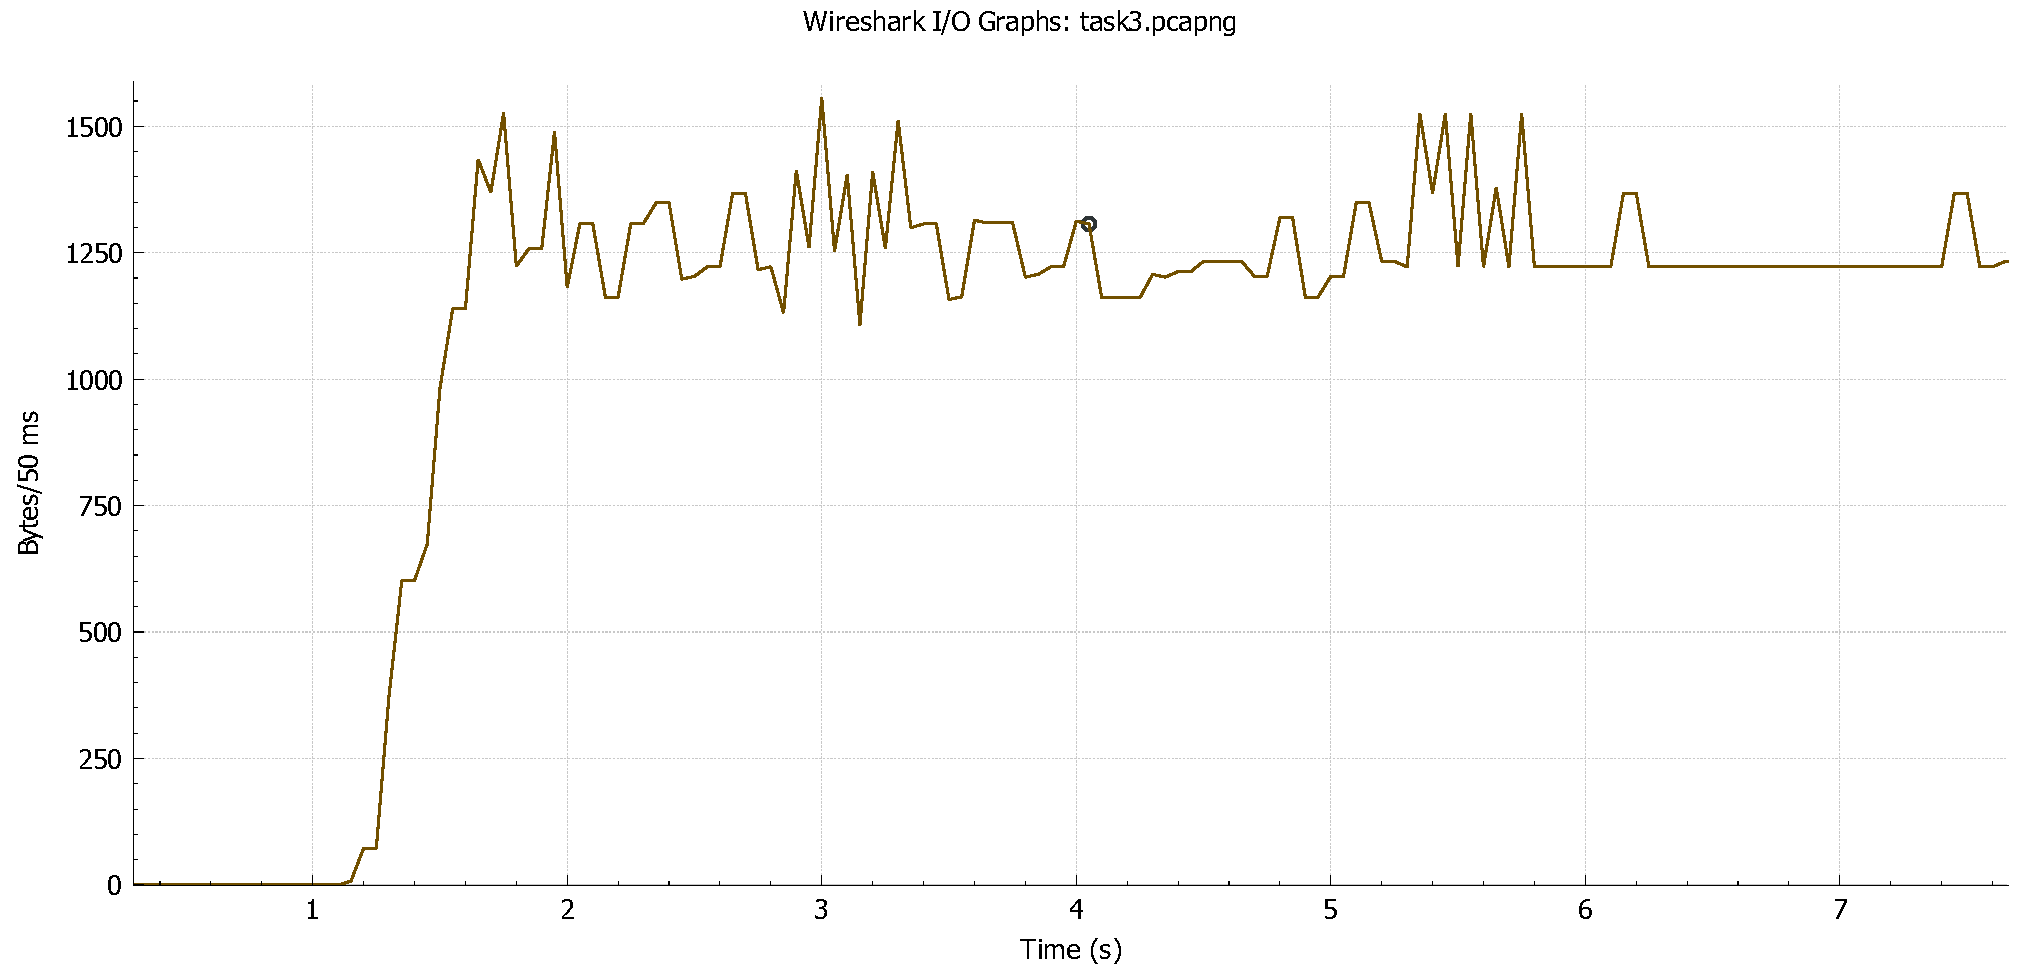
\includegraphics[width=0.8\textwidth]{io.pdf}
\end{figure}
从I/O图中可以看出首先,每秒传播的字节数按照指数级增长,然后按照线性增长。
后来有一些下降的过程,然后快速地增长,大致对应了慢启动、拥塞避免和快速重传的过程。
此外,借助Wireshark绘制吞吐量图如图~\ref{fig:tp}。
\begin{figure}[htb]
	\centering
	\caption{吞吐量图}
	\label{fig:tp}
	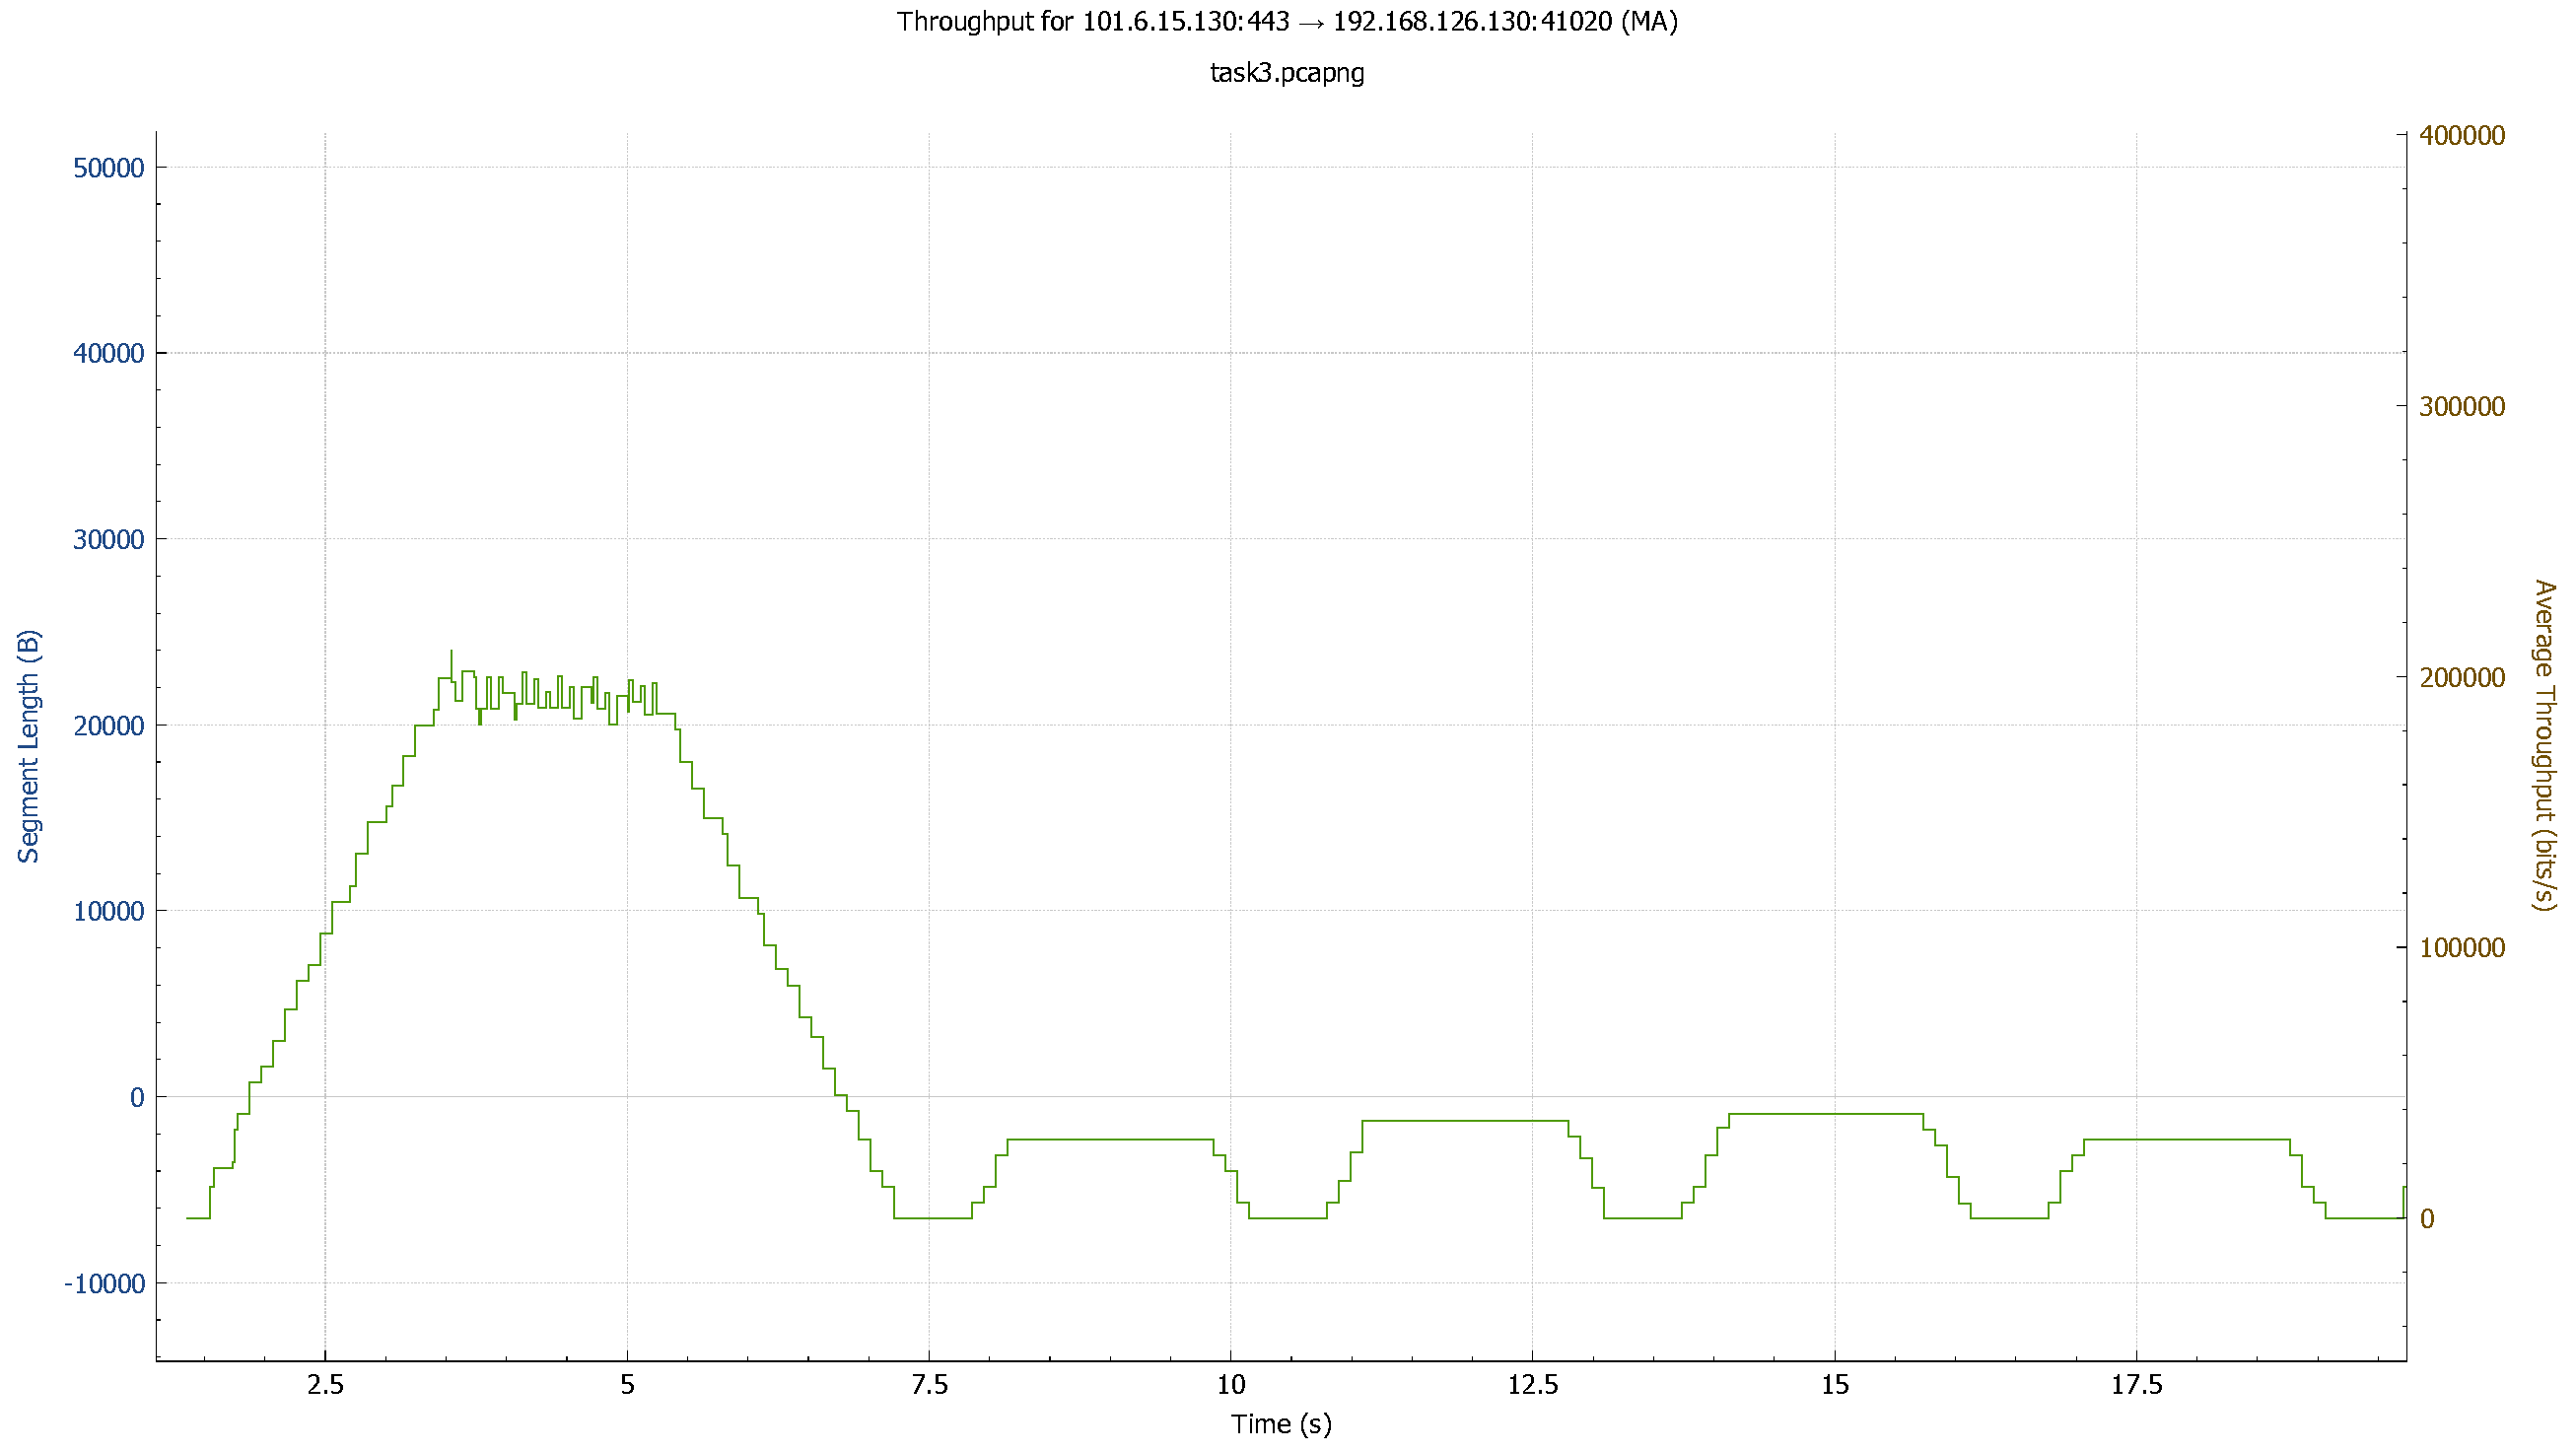
\includegraphics[width=0.8\textwidth]{tp.pdf}
\end{figure}
可以发现也遵循了类似的变化过程。

例如2秒左右时发生的快速重传,首先由于链路带宽的问题,客户端收到了不正常的序列号,因此启动了快重传
机制。如图~\ref{fig:dupack}所示。
\begin{figure}[htb]
	\centering
	\caption{DupACK}
	\label{fig:dupack}
	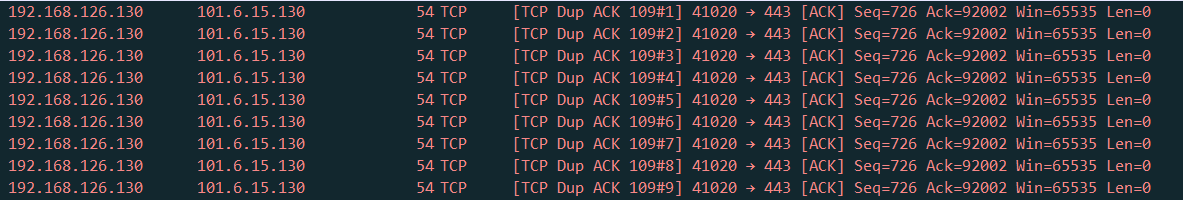
\includegraphics[width=0.6\textwidth]{dupack.png}
\end{figure}
由于Duplicate Ack的存在,服务器端重传了相应的报文,如图~\ref{fig:dupack2}所示。
\begin{figure}[htb]
	\centering
	\caption{重传}
	\label{fig:dupack2}
	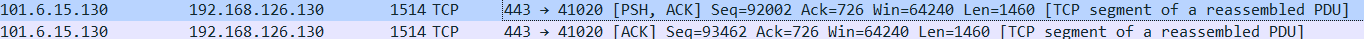
\includegraphics[width=0.6\textwidth]{retra.png}
\end{figure}
此时重传的报文还加入了PSH标志,让客户端尽快交付。从图~\ref{fig:io}中可以观察到,
虽然由于重传$cwnd$减少了,但是由于快重传机制,$cwnd$开始快速回复了,进行了
指数级的增长。


\section{任务4、HTTP协议分析}

\subsection{实验准备}

\texttt{http.server}库提供直接使用命令行的方式启动HTTP服务器,但是早期版本不方便
切换协议,因此先把python版本升级到3.11,如图~\ref{fig:py11}所示。
\begin{figure}[htb]
	\centering
	\caption{升级python版本}
	\label{fig:py11}
	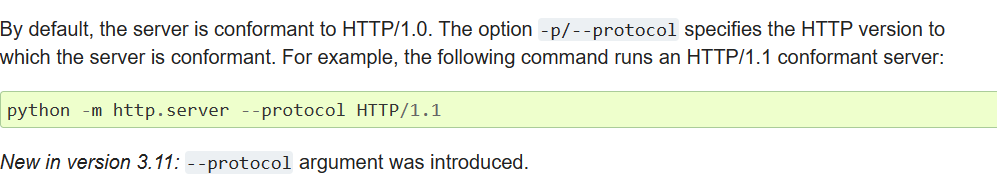
\includegraphics[width=0.6\textwidth]{py11.png}
\end{figure}

这样就可以用\texttt{--protocol}参数直接指定协议了,方便了后续的实验。

\subsection{实验结果}

实验结果如图~\ref{fig:http}所示。图~\ref{fig:http10}显示了HTTP1.0多次请求的结果,
由于HTTP1.0不支持持久连接,因此每次请求都需要重新建立连接。可以看到,每次请求都先包含了
TCP的三次握手。在请求结束后都包含了TCP的四次挥手。这样多次建立连接,既浪费了几个RTT的时间,
又浪费了服务器端的资源。

\begin{figure}[H]
	\centering
	\caption{不同版本的HTTP}
	\label{fig:http}
	\begin{subfigure}{0.4\textwidth}
		\centering
		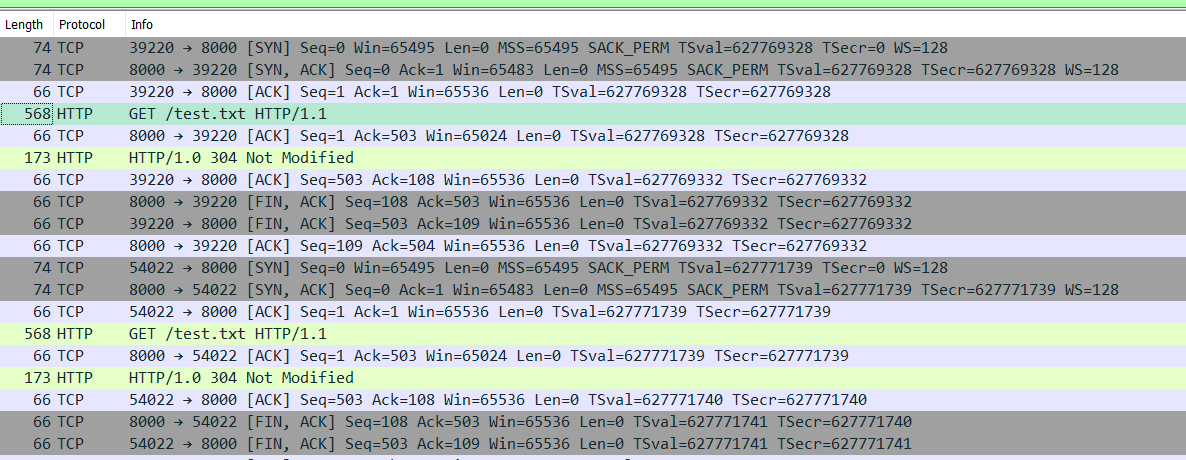
\includegraphics[width=\textwidth]{http10.png}
		\caption{HTTP1.0}
		\label{fig:http10}
	\end{subfigure}
	\begin{subfigure}{0.4\textwidth}
		\centering
		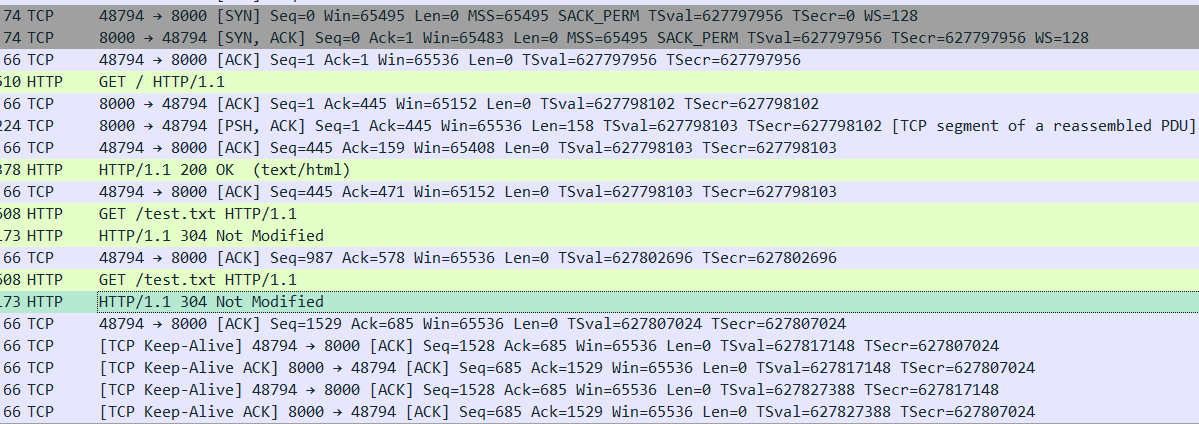
\includegraphics[width=\textwidth]{http11.png}
		\caption{HTTP1.1}
		\label{fig:http11}
	\end{subfigure}
	\begin{subfigure}{0.4\textwidth}
		\centering
		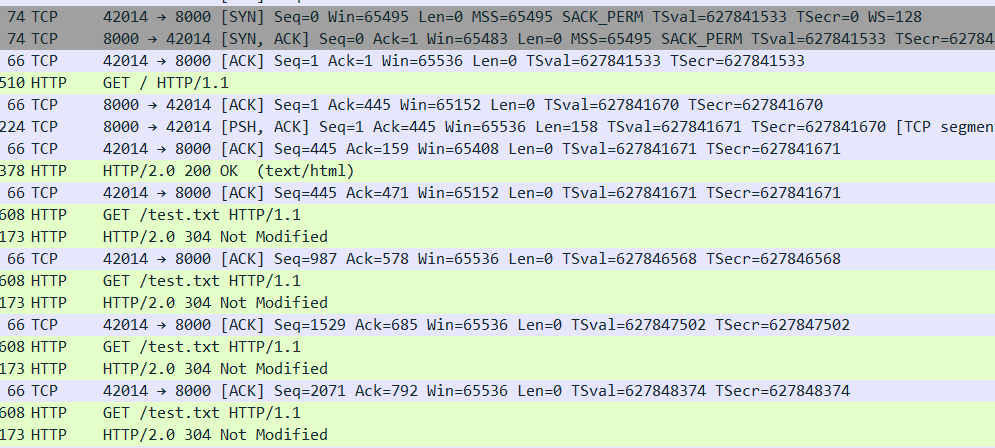
\includegraphics[width=\textwidth]{http20.png}
		\caption{HTTP2.0}
		\label{fig:http20}
	\end{subfigure}
\end{figure}

图~\ref{fig:http11}显示了HTTP1.1多次请求的结果。由于HTTP1.1支持持久连接,y因此只有一开始
有三次握手,后面的请求都是直接使用相同的TCP连接发送数据。这样就大大减少了开销。为了让服务器
判断是否需要继续保持连接,HTTP1.1也会发送Keep-Alive的请求头,让服务器判断是否需要保持连接。
可以看到发送的信息中也有一些TCP Keep-Alive的信息,这些信息是用来维持TCP连接的。

图~\ref{fig:http20}显示了HTTP2多次请求的结果。由于HTTP2是基于TCP的,因此也是需要三次握手。
HTTP2.0的多路复用机制,可以让多个请求共享一个TCP连接,因此可以看到所有请求都使用了客户机42014
端口打开的TCP连接。这大大节省了服务器的资源,也减少了开销。

\end{spacing}

\end{document}